\documentclass[
11pt, % The default document font size, options: 10pt, 11pt, 12pt
%codirector, % Uncomment to add a codirector to the title page
]{charter} 


% El títulos de la memoria, se usa en la carátula y se puede usar el cualquier lugar del documento con el comando \ttitle
\titulo{Desarrollo de hardware y firmware para un sistema de control, gestión y comunicación de luminaria pública} 

% Nombre del posgrado, se usa en la carátula y se puede usar el cualquier lugar del documento con el comando \degreename
\posgrado{Carrera de Especialización en Sistemas Embebidos} 
%\posgrado{Carrera de Especialización en Internet de las Cosas} 
%\posgrado{Carrera de Especialización en Inteligencia Artificial}
%\posgrado{Maestría en Sistemas Embebidos} 
%\posgrado{Maestría en Internet de las cosas}
% IMPORTANTE: no omitir titulaciones ni tildación en los nombres, también se recomienda escribir los nombres completos (tal cual los tienen en su documento)
% Tu nombre, se puede usar el cualquier lugar del documento con el comando \authorname
\autor{Ing. Juan Manuel Guariste}

% El nombre del director y co-director, se puede usar el cualquier lugar del documento con el comando \supname y \cosupname y \pertesupname y \pertecosupname
\director{Ing. Juan Manuel Cruz}
\pertenenciaDirector{FIUBA} 
\codirector{} % para que aparezca en la portada se debe descomentar la opción codirector en los parámetros de documentclass
%\pertenenciaCoDirector{FIUBA}

% Nombre del cliente, quien va a aprobar los resultados del proyecto, se puede usar con el comando \clientename y \empclientename
\cliente{Ing. Bernardo Martínez Sáenz}
\empresaCliente{Deitres S.A.}
 
\fechaINICIO{20 de agosto de 2024}		%Fecha de inicio de la cursada de GdP \fechaInicioName
\fechaFINALPlan{8 de octubre de 2024} 	%Fecha de final de cursada de GdP
\fechaFINALTrabajo{junio de 2025}	%Fecha de defensa pública del trabajo final


\begin{document}

\maketitle
\thispagestyle{empty}
\pagebreak


\thispagestyle{empty}
{\setlength{\parskip}{0pt}
\tableofcontents{}
}
\pagebreak


\section*{Registros de cambios}
\label{sec:registro}


\begin{table}[ht]
\label{tab:registro}
\centering
\begin{tabularx}{\linewidth}{@{}|c|X|c|@{}}
\hline
\rowcolor[HTML]{C0C0C0} 
Revisión & \multicolumn{1}{c|}{\cellcolor[HTML]{C0C0C0}Detalles de los cambios realizados} & Fecha      \\ \hline
0      & Creación del documento                                 &\fechaInicioName \\ \hline
1      & Se completa hasta el punto 5 inclusive           & 3 de septiembre de 2024 \\ \hline
2      & Se completa hasta el punto 9 inclusive	       & 10 de septiembre de 2024 \\ \hline
%		  Se puede agregar algo más \newline
%		  En distintas líneas \newline
%		  Así                                                    & {día} de {mes} de 202X \\ \hline
%3      & Se completa hasta el punto 12 inclusive                & {día} de {mes} de 202X \\ \hline
%4      & Se completa el plan	                                 & {día} de {mes} de 202X \\ \hline

% Si hay más correcciones pasada la versión 4 también se deben especificar acá

\end{tabularx}
\end{table}

\pagebreak



\section*{Acta de constitución del proyecto}
\label{sec:acta}

\begin{flushright}
Buenos Aires, \fechaInicioName
\end{flushright}

\vspace{2cm}

%Por medio de la presente se acuerda con el \authorname\hspace{1px} que su Trabajo Final de la \degreename\hspace{1px} se titulará ``\ttitle'' y consistirá en \textcolor{red}{la implementación de un prototipo de un sistema de control de temperatura de una caldera industrial}. El trabajo tendrá un presupuesto preliminar estimado de \textcolor{red}{600} horas y un costo estimado de \textcolor{red}{U\$D 1000}, con fecha de inicio el \fechaInicioName\hspace{1px} y fecha de presentación pública el \fechaFinalName.

%Se adjunta a esta acta la planificación inicial.

Por medio de la presente se acuerda con el \authorname\hspace{1px} que su Trabajo Final de la \degreename\hspace{1px} se titulará ``\ttitle'' y consistirá en la implementación de un prototipo para el control eficiente y remoto de las luminarias, permitiendo una comunicación efectiva y robusta entre ellas y una gestión centralizada. El trabajo tendrá un presupuesto preliminar estimado de 600 horas y un costo estimado de U\$D 1000, con fecha de inicio el \fechaInicioName\hspace{1px} y fecha de presentación pública en \fechaFinalName.

Se adjunta a esta acta la planificación inicial.

\vfill

% Esta parte se construye sola con la información que hayan cargado en el preámbulo del documento y no debe modificarla
\begin{table}[ht]
\centering
\begin{tabular}{ccc}
\begin{tabular}[c]{@{}c@{}}Dr. Ing. Ariel Lutenberg \\ Director posgrado FIUBA\end{tabular} & \hspace{2cm} & \begin{tabular}[c]{@{}c@{}}\clientename \\ \empclientename \end{tabular} \vspace{2.5cm} \\ 
\multicolumn{3}{c}{\begin{tabular}[c]{@{}c@{}} \supname \\ Director del Trabajo Final\end{tabular}} \vspace{2.5cm} \\
\end{tabular}
\end{table}




\section{1. Descripción técnica-conceptual del proyecto a realizar}
\label{sec:descripcion}

El proyecto está alineado con las necesidades de Deitres S.A., empresa donde el autor de este proyecto trabaja como ingeniero de desarrollo de hardware y firmware. Deitres S.A. se especializa en crear soluciones tecnológicas e innovadoras para la seguridad electrónica, domótica y la industria. Este proyecto aborda la ineficiencia en la gestión de la iluminación pública, un problema crítico en las ciudades modernas donde el control efectivo y el ahorro energético son esenciales. Muchas ciudades enfrentan dificultades para mantener un control preciso sobre sus redes de iluminación pública, lo que genera altos costos operativos, de mantenimiento y de consumo energético.

Actualmente, existen diversas soluciones para la gestión de la iluminación pública, desde sistemas básicos de encendido y apagado programado hasta tecnologías más avanzadas que permiten el control remoto y la automatización. Sin embargo, muchas de estas soluciones tienen limitaciones en términos de escalabilidad, robustez de comunicación y capacidad de integración con otras tecnologías.

La solución propuesta es el CityLight, un prototipo de luminaria inteligente que se conecta a Internet a través de Wi-Fi y redes celulares. Estos dispositivos, una vez instalados, interactúan entre sí formando una red con topología mesh en 915 MHz, utilizando un protocolo propio desarrollado por la empresa e implementado en otros de sus productos. Si un dispositivo necesita comunicar un evento o el estado de una luminaria y no cuenta con conexión a Internet, podrá utilizar esta red mesh para conectarse con otro CityLight que funcione como gateway. Esto no solo garantiza un sistema de comunicación eficiente y robusto, sino que también ofrece la ventaja de superar una eventual obsolescencia tecnológica. Por ejemplo, si en una ciudad se desmantelan las redes celulares 3G, los CityLight que utilizaban esa interfaz de conexión a Internet podrán seguir comunicando sus eventos a través de la red mesh, conectándose a otros CityLight con otras formas de conexión, como Wi-Fi. Además, si surge una nueva tecnología de conexión a Internet, como la satelital o 5G, bastará con que un solo CityLight disponga de esa interfaz para que pueda actuar como gateway para los demás nodos de la red mesh.

A continuación, se detallan las funcionalidades específicas que se implementarán en el prototipo de luminaria inteligente, CityLight:

\begin{itemize}
		\item \textbf{Conector NEMA:} dispondrá de una interfaz física NEMA para conectarse a las luminarias, permitiendo una integración estándar con diversos sistemas de iluminación existentes.
        \item \textbf{Medición de intensidad lumínica ambiental mediante sensor fotosensible (fotocélula)}: permitirá ajustar la iluminación en función de las condiciones de luz externa.
        \item \textbf{Actuación sobre la intensidad lumínica de la luminaria mediante circuito dimmer}: facilitará el ajuste de la intensidad de la luz según las necesidades.
        \item \textbf{Medición de consumo de corriente AC}: para monitorear el consumo energético de las luminarias.
        \item \textbf{Detección de presencia de tensión AC}: para asegurar el correcto funcionamiento del sistema.
        \item \textbf{Utilización de circuito adaptador de señales para control de la luminaria}: adaptará las señales de control.
        \item \textbf{Control de habilitación/deshabilitación de suministro de corriente a la luminaria mediante accionamiento de relé}: permitirá encender o apagar las luminarias de manera automatizada o por comandos enviados remotamente.
        \item \textbf{Interfaz de conexión a Internet}: el sistema podrá recibir comandos y enviar reportes a través de interfaces Wi-Fi y celular. Se le podrá consultar el estado de la luminaria y actuar sobre ella.
        \item \textbf{Red mesh}: implementación de la red mesh en 915 MHz que permita la comunicación entre dispositivos CityLight. 
        \item \textbf{Geo-posicionamiento de luminarias}: utilización de GPS para la localización precisa de cada unidad.
        \item \textbf{Posibilidad de operar con alimentación alterna o a batería}:  asegurará la operación del sistema bajo diversas condiciones de suministro energético.
\end{itemize}

En la figura \ref{fig:diagBloquesGeneral}, se presenta un diagrama en bloques del sistema propuesto en el que se observan las distintas funcionalidades a implementar. 

\begin{figure}[htpb]
\centering 
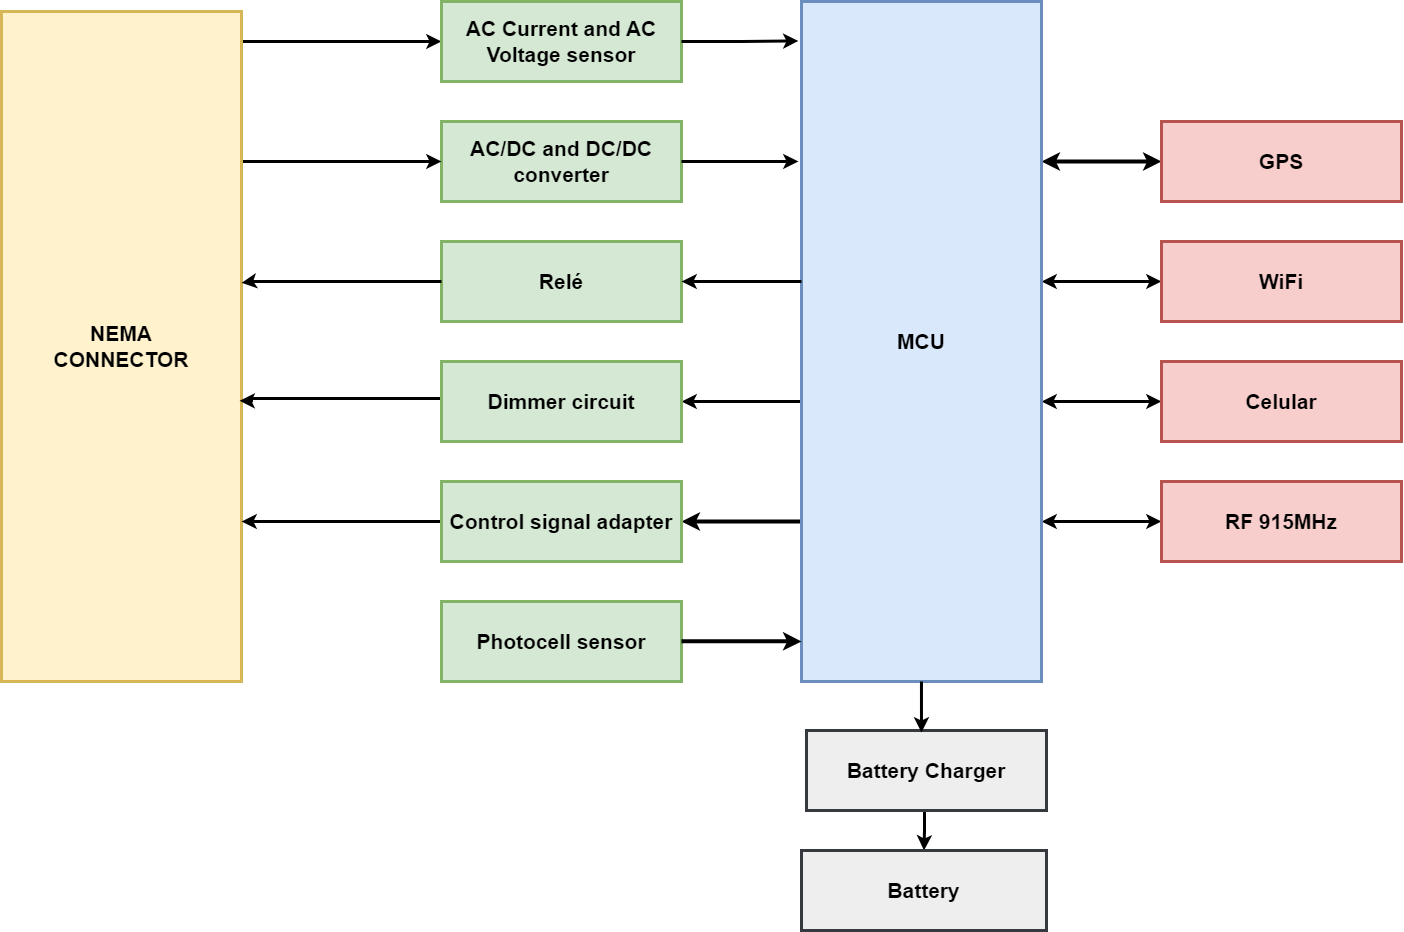
\includegraphics[width=.9\textwidth]{./Figuras/diagBloquesGeneral.png}
\caption{Diagrama en bloques del sistema.}
\label{fig:diagBloquesGeneral}
\end{figure}

El cliente de este proyecto valora la aplicación de la red mesh en 915 MHz debido a su éxito en otros productos desarrollados por la empresa. La integración de esta red distingue al proyecto CityLight de otras soluciones, ofreciendo una comunicación más robusta y eficiente entre las luminarias y mejorando la escalabilidad del sistema. Este proyecto es crucial para Deitres S.A. porque permitirá expandir el uso de una tecnología ya validada y apreciada, reforzando su posición en el mercado de soluciones para la gestión de infraestructuras urbanas.

 \pagebreak

\section{2. Identificación y análisis de los interesados}
\label{sec:interesados}

\begin{table}[ht]
%\caption{Identificación de los interesados}
%\label{tab:interesados}
\begin{tabularx}{\linewidth}{@{}|l|X|X|p{5cm}|@{}}
\hline
\rowcolor[HTML]{C0C0C0} 
Rol           & Nombre y Apellido & Organización 	& Puesto 	\\ \hline
%Auspiciante   &                   &              	&        	\\ \hline
Cliente       & \clientename      &\empclientename	&CEO de Deitres S.A.      	\\ \hline
%Impulsor      &                   &              	&        	\\ \hline
Responsable   & \authorname       & FIUBA        	& Alumno 	\\ \hline
Colaboradores &       Gustavo Vasoin  \newline Ing. Daniel Alejandro Ismael          &      Deitres S.A.  \newline Deitres S.A. 	&   Desarrollador de firmware \newline  Desarrollador de hardware y firmware\\ \hline
Orientador    & \supname	      & \pertesupname 	& Director del Trabajo Final \\ \hline
%Equipo        & miembro1 \newline 
%				miembro2          &              	&        	\\ \hline
%Opositores    &                   &              	&        	\\ \hline
Usuario final &Municipalidades y empresas de infraestructura urbana         &-              	&-        	\\ \hline
\end{tabularx}
\end{table}

Cliente: el Ing. Bernardo Martínez Sáenz es un líder con amplia experiencia en el sector de la seguridad electrónica y la domótica. Su visión estratégica en la implementación de soluciones innovadoras será fundamental para guiar el desarrollo del proyecto CityLight.

Orientador: el Ing. Juan Manuel Cruz es un profesional de alta capacidad técnica y de gestión, con una destacada trayectoria en el ámbito de sistemas embebidos. Sus observaciones y recomendaciones serán fundamentales para el éxito del proyecto, ya que aportará no solo su experiencia técnica, sino también su visión estratégica para guiar el desarrollo y asegurar que se alcancen los objetivos propuestos.

Colaboradores: Gustavo Vasoin es un profesional con una sólida trayectoria en el desarrollo de firmware para sistemas embebidos. El Ing. Daniel Alejandro Ismael, con amplia experiencia en el  diseño y desarrollo de hardware y firmware, aporta un enfoque integral en la creación de sistemas electrónicos. Ambos trabajan en la empresa para la cual se desarrolla el producto. Su experiencia y conocimientos técnicos serán fundamentales para lograr un producto de alta calidad, cumpliendo con los estándares de innovación y eficiencia que demanda el proyecto.

\section{3. Propósito del proyecto}
\label{sec:proposito}

Mejorar la eficiencia en la gestión de la iluminación pública, reducir los costos operativos y de mantenimiento, y optimizar el consumo energético. Se busca desarrollar un sistema de luminarias inteligentes con conexión a Internet que permita un control preciso y remoto, garantizando una comunicación robusta y escalable entre las luminarias mediante una red mesh.

\section{4. Alcance del proyecto}
\label{sec:alcance}

El proyecto incluye el diseño de circuito impreso y desarrollo de firmware que permita:
\begin{itemize}
	\item Conexión con el conector NEMA.
	\item Adquisición de señales y control de la luminaria.
	\item Implementar interfaces de conexión a Internet mediante Wi-Fi y red celular.
	\item Geolocalización mediante modulo GPS.
	\item Implementación de red mesh en 915 MHz.
	\item Integración del CityLight con el software de control y gestión existente en la empresa.
\end{itemize}	

El proyecto no incluye:
\begin{itemize}
	\item Desarrollo de nuevo software de control y gestión para los dispositivos.
	\item Pruebas de campo del prototipo.
	\item Certificación del prototipo ante organismos regulatorios nacionales y/o internacionales.
\end{itemize}


\section{5. Supuestos del proyecto}
\label{sec:supuestos}


Para el desarrollo del presente proyecto se supone que: 

\begin{itemize}
	\item El Ing. Juan Manuel Guariste, responsable del proyecto, y el Ing. Bernardo Martínez Sáenz, cliente del proyecto, estan de acuerdo con los requerimientos y 		alcance planteado en este documento.
	\item El presupuesto necesario para el desarrollo estará a cargo de la empresa Deitres S. A.
	\item El Ing. Juan Manuel Guariste dispondrá eventualmente de tiempo de la jornada laboral para llevar a cabo el proyecto en el plazo especificado en el acta de constitución.
	\item Se conseguirán todos los componentes necesarios para el desarrollo en tiempo y forma.	
	%\item Se dispondrá del instrumental de laboratorio adecuado para realizar mediciones al prototipo.
	\item En caso de no contar con algún conocimiento específico para desarrollar el proyecto, se podrá contar con el apoyo o soporte del cuerpo docente de la especialización.
\end{itemize}


\section{6. Requerimientos}
\label{sec:requerimientos}

\begin{enumerate}
	\item Requerimientos asociados con el hardware:
		\begin{enumerate}
			\item El sistema debe contar con una interfaz física NEMA de 7 pines para conectarse y comunicarse con las luminarias de alumbrado público.
			\item La implementación debe ser compatible con una carcasa genérica para luminarias.
			\item  El sistema debe integrar un sensor de efecto hall para medir el consumo de corriente AC de la luminaria conectada.
			\item El sistema debe detectar la presencia de tensión AC en la luminaria utilizando un optoacoplador.
 			\item El sistema debe ser capaz de regular la intensidad lumínica de la luminaria a través de un circuito dimmer.
			\item Debe contar con un sensor fotosensible que mida la intensidad lumínica ambiental.
			%\item Debe poseer circuitería de adaptación de señales de control.
			\item El sistema debe integrar un relé para controlar la habilitación o deshabilitación del suministro de corriente a la luminaria.
			\item Debe tener conectividad a internet mediante un módulo Wi-Fi.
			\item Debe tener conectividad a internet mediante red celular.
			\item El sistema debe integrar un transceptor en la banda de 915 MHz para establecer y mantener la red mesh de luminarias.
			\item Se debe utilizar un amplificador para el transceptor de 915 MHz que permita aumentar la potencia de salida al menos 20 dBm.
			\item El sistema debe incluir un módulo GPS para obtener la posición geográfica de cada luminaria y sincronizar datos como la hora y ubicación precisa.
			\item Debe ser capaz de operar tanto con alimentación de la red eléctrica como a través de una batería en caso de cortes o fallos en el suministro eléctrico. 
			\item La conmutación entre la alimentación de la red eléctrica y la batería debe ser automáticamente mediante circuitos analógicos, garantizando la continuidad sin intervención manual.
			\item Se debe implementar un circuito de carga de batería que permita su recarga segura cuando el sistema esté conectado a la red eléctrica.
			\item Se debe implementar circuitos de adaptación de señales para medir la tension de batería con el ADC.
		\end{enumerate}

	\item Requerimientos asociados con el firmware:
		\begin{enumerate}		
		\item El firmware debe estar implementado sobre un sistema operativo de tiempo real (RTOS), asegurando el manejo eficiente de múltiples tareas críticas como control, monitoreo y comunicación.
		\item Se debe implementar el protocolo de comunicación para la red mesh utilizando el transceptor de 915 MHz.
		\item EL sistema debe implementar la interfaz de conexión a internet a través del módulo Wi-Fi, permitiendo al sistema enviar y recibir datos desde plataformas de gestión remota.
		\item Debe implementar la interfaz de conexión a internet a través del módulo celular, permitiendo al sistema enviar y recibir datos desde plataformas de gestión remota.
		\item El firmware debe incluir la lógica de selección de conexión a internet, priorizando la interfaz Wi-Fi cuando ambas conexiones estén disponibles, y conmutando a celular en caso de fallo.
		\item En caso de no disponer conexión a internet, el sistema debe utilizar la red mesh para comunicarse con un gateway presente en la red, que será el encargado de enviar y recibir datos hacia y desde internet. 
		\item El firmware debe procesar y gestionar los datos proporcionados por el sensor fotosensible.
		\item El sistema debe permitir el encendido automático de las luminarias según los niveles de luz ambiental detectados, o mediante comandos remotos.
		\item Debe ser posible la actualización del firmware over-the-air (OTA).
		\item El firmware debe controlar la intensidad lumínica de las luminarias, regulando la tensión de entrada del circuito dimmer a través del firmware.
		\item El firmware debe procesar la información del módulo GPS para geoposicionamiento y sincronización horaria.
		\item Se debe procesar e informar los datos de consumo eléctrico enviados por el sensor de efecto hall.
		\item El firmware debe procesar los datos enviados por el optoacoplador para detectar la presencia o ausencia de tensión alterna en la luminaria.
		\item Debe medir y reportar la tensión de la batería utilizando el ADC.
		\end{enumerate}
\end{enumerate}

\section{7. Historias de usuarios (\textit{Product backlog})}
\label{sec:backlog}

\begin{consigna}{red}
Descripción: en esta sección se deben incluir las historias de usuarios y su ponderación (\textit{history points}). Recordar que las historias de usuarios son descripciones cortas y simples de una característica contada desde la perspectiva de la persona que desea la nueva capacidad, generalmente un usuario o cliente del sistema. La ponderación es un número entero que representa el tamaño de la historia comparada con otras historias de similar tipo.

Se debe indicar explícitamente el criterio para calcular los \textit{story points} de cada historia.

El formato propuesto es: 
\begin{enumerate}
\item ``Como [rol] quiero [tal cosa] para [tal otra cosa]."

\textit{Story points}: 8 (complejidad: 3, dificultad: 2, incertidumbre: 3)
\end{enumerate}
\end{consigna}

\section{8. Entregables principales del proyecto}
\label{sec:entregables}

\begin{consigna}{red}
Los entregables del proyecto son (ejemplo):

\begin{itemize}
	\item Manual de usuario.
	\item Diagrama de circuitos esquemáticos.
	\item Código fuente del firmware.
	\item Diagrama de instalación.
	\item Memoria del trabajo final.
	\item etc...
\end{itemize}
\end{consigna}

\section{9. Desglose del trabajo en tareas}
\label{sec:wbs}

\begin{consigna}{red}
El WBS debe tener relación directa o indirecta con los requerimientos.  Son todas las actividades que se harán en el proyecto para dar cumplimiento a los requerimientos. Se recomienda mostrar el WBS mediante una lista indexada:

\begin{enumerate}
\item Grupo de tareas 1 (suma h)
	\begin{enumerate}
	\item Tarea 1 (tantas h)
	\item Tarea 2 (tantas h)
	\item Tarea 3 (tantas h)
	\end{enumerate}
\item Grupo de tareas 2 (suma h)
	\begin{enumerate}
	\item Tarea 1 (tantas h)
	\item Tarea 2 (tantas h)
	\item Tarea 3 (tantas h)
	\end{enumerate}
\item Grupo de tareas 3 (suma h)
	\begin{enumerate}
	\item Tarea 1 (tantas h)
	\item Tarea 2 (tantas h)
	\item Tarea 3 (tantas h)
	\item Tarea 4 (tantas h)
	\item Tarea 5 (tantas h)
	\end{enumerate}
\end{enumerate}

Cantidad total de horas: tantas.

\textbf{¡Importante!:} la unidad de horas es h y va separada por espacio del número. Es incorrecto escribir ``23hs".

\textbf{Se recomienda que no haya ninguna tarea que lleve más de 40 h.} De ser así se recomienda dividirla en tareas de menor duración.

\end{consigna}

\section{10. Diagrama de Activity On Node}
\label{sec:AoN}

\begin{consigna}{red}
Armar el AoN a partir del WBS definido en la etapa anterior.

Una herramienta simple para desarrollar los diagramas es el Draw.io (\url{https://app.diagrams.net/}).
\href{https://app.diagrams.net}{Draw.io}


\begin{figure}[htpb]
\centering 
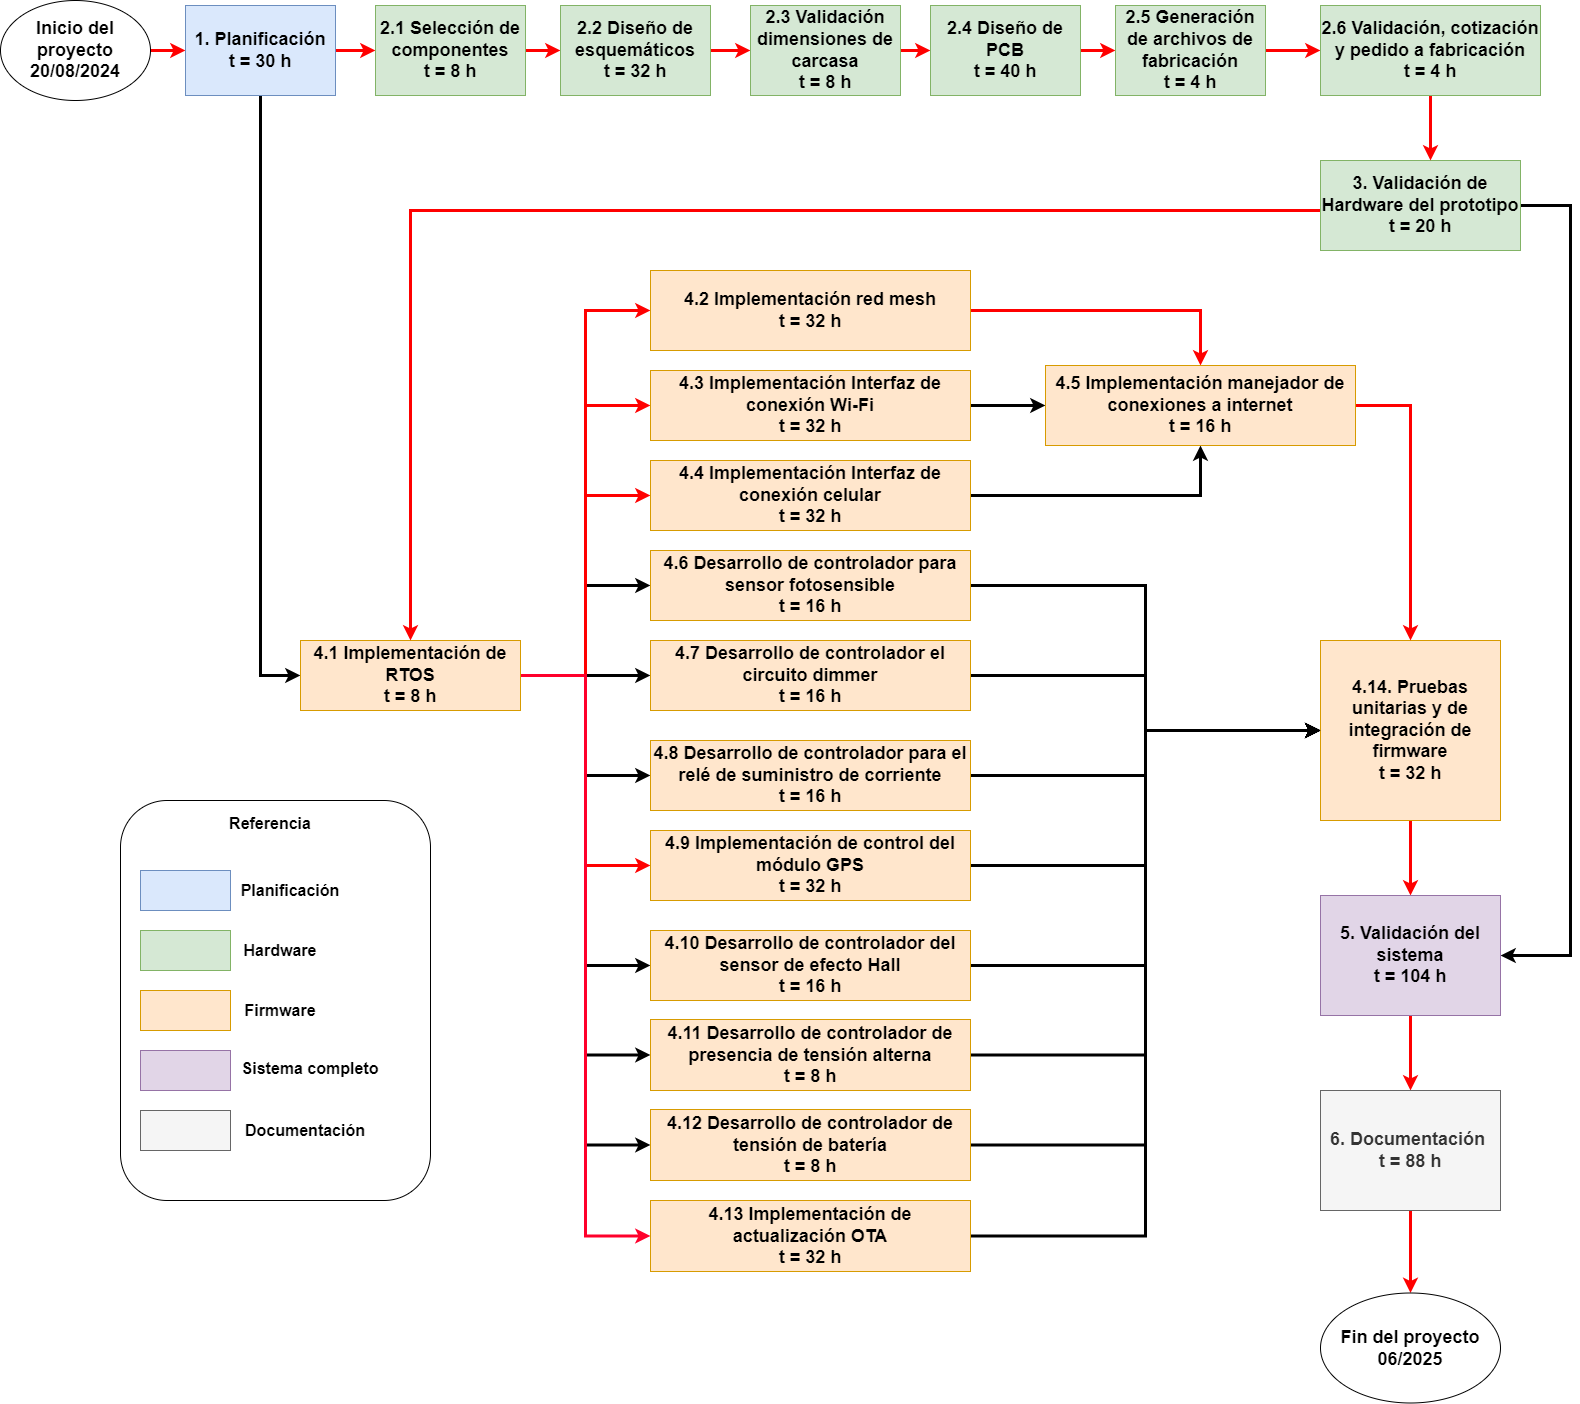
\includegraphics[width=.8\textwidth]{./Figuras/AoN.png}
\caption{Diagrama de \textit{Activity on Node}.}
\label{fig:AoN}
\end{figure}

Indicar claramente en qué unidades están expresados los tiempos.
De ser necesario indicar los caminos semi críticos y analizar sus tiempos mediante un cuadro.
Es recomendable usar colores y un cuadro indicativo describiendo qué representa cada color.

\end{consigna}

\section{11. Diagrama de Gantt}
\label{sec:gantt}

\begin{consigna}{red}
Existen muchos programas y recursos \textit{online} para hacer diagramas de Gantt, entre los cuales destacamos:

\begin{itemize}
\item Planner
\item GanttProject
\item Trello + \textit{plugins}. En el siguiente link hay un tutorial oficial: \\ \url{https://blog.trello.com/es/diagrama-de-gantt-de-un-proyecto}
\item Creately, herramienta online colaborativa. \\\url{https://creately.com/diagram/example/ieb3p3ml/LaTeX}
\item Se puede hacer en latex con el paquete \textit{pgfgantt}\\ \url{http://ctan.dcc.uchile.cl/graphics/pgf/contrib/pgfgantt/pgfgantt.pdf}
\end{itemize}

Pegar acá una captura de pantalla del diagrama de Gantt, cuidando que la letra sea suficientemente grande como para ser legible. 
Si el diagrama queda demasiado ancho, se puede pegar primero la ``tabla'' del Gantt y luego pegar la parte del diagrama de barras del diagrama de Gantt.

Configurar el software para que en la parte de la tabla muestre los códigos del EDT (WBS).\\
Configurar el software para que al lado de cada barra muestre el nombre de cada tarea.\\
Revisar que la fecha de finalización coincida con lo indicado en el Acta Constitutiva.

En la figura \ref{fig:gantt}, se muestra un ejemplo de diagrama de gantt realizado con el paquete de \textit{pgfgantt}. 
En la plantilla pueden ver el código que lo genera y usarlo de base para construir el propio.

Las fechas pueden ser calculadas utilizando alguna de las herramientas antes citadas. Sin embargo, el siguiente ejemplo
fue elaborado utilizando 
\href{https://docs.google.com/spreadsheets/d/1fBz8NhSpc4tkkhz3KjJCbh1nR_ltDkfEcZi4tZXduqs}{esta hoja de cálculo}.

Es importante destacar que el ancho del diagrama estará dado por la longitud del texto utilizado para las tareas 
(Ejemplo: tarea 1, tarea 2, etcétera) y el valor \textit{x unit}. Para mejorar la apariencia del diagrama, es necesario
ajustar este valor y, quizás, acortar los nombres de las tareas.

\begin{figure}[htpb]
  \begin{center}
    \begin{ganttchart}[
      time slot unit=day,
      time slot format=isodate,
      x unit=0.038cm,
      y unit title=0.7cm,
      y unit chart=0.6cm,
      milestone/.append style={xscale=4}
      ]{2021-03-05}{2021-12-16}
      \gantttitlecalendar*{2021-03-05}{2021-12-16}{year} \\
      \gantttitlecalendar*{2021-03-05}{2021-12-16}{month} \\
      \ganttgroup{Duración Total}{2021-03-05}{2021-12-16} \\
      %%%%%%%%%%%%%%%%%Organización
      \ganttgroup{Organización}{2021-03-05}{2021-04-16} \\
      \ganttbar{Planificación del proyecto}{2021-03-05}{2021-04-15} \\
      %%%%%%%%%%%%%%%%%Ejecución
      \ganttgroup{Ejecución}{2021-04-16}{2021-10-21} \\
      \ganttbar{Tarea 1}{2021-04-16}{2021-04-29} \\
      \ganttbar{Tarea 2}{2021-04-30}{2021-05-13} \\
      \ganttbar{Tarea 3}{2021-05-14}{2021-05-27} \\
      \ganttbar{Tarea 4}{2021-05-28}{2021-07-12} \\
      \ganttbar{Tarea 5}{2021-07-13}{2021-08-09} \\
      \ganttbar{Tarea 6}{2021-08-10}{2021-09-23} \\
      \ganttbar{Tarea 7}{2021-09-24}{2021-09-30} \\
      \ganttbar{Tarea 8}{2021-10-01}{2021-10-14} \\
      \ganttbar{Tarea 9}{2021-10-15}{2021-10-21} \\
      % %%%%%%%%%%%%%%%%%Finalización
      \ganttgroup{Finalización}{2021-10-22}{2021-12-16} \\
      \ganttbar{Memoria v1}{2021-10-22}{2021-11-04} \\
      \ganttbar{Memoria v2}{2021-11-05}{2021-11-18} \\
      \ganttbar{Memoria final}{2021-11-19}{2021-12-02} \\
      % La fecha del siguiente milestone es la fecha en que terminamos la memoria
      \ganttmilestone{Enviar memoria al director}{2021-12-02} \\
      \ganttbar{Elaborar la presentación}{2021-12-03}{2021-12-16} \\
      \ganttmilestone{Ensayo de la presentación}{2021-12-16} \\
      %%%%%%%%%%%%%%%%%%%%%%%%%%%%%%%%%%%%%%%%%%%%%%%%%%%%%%%%%%%%%%%
    \end{ganttchart}
  \end{center}
  \caption{Diagrama de gantt de ejemplo}
  \label{fig:gantt}
\end{figure}


\begin{landscape}
\begin{figure}[htpb]
\centering 
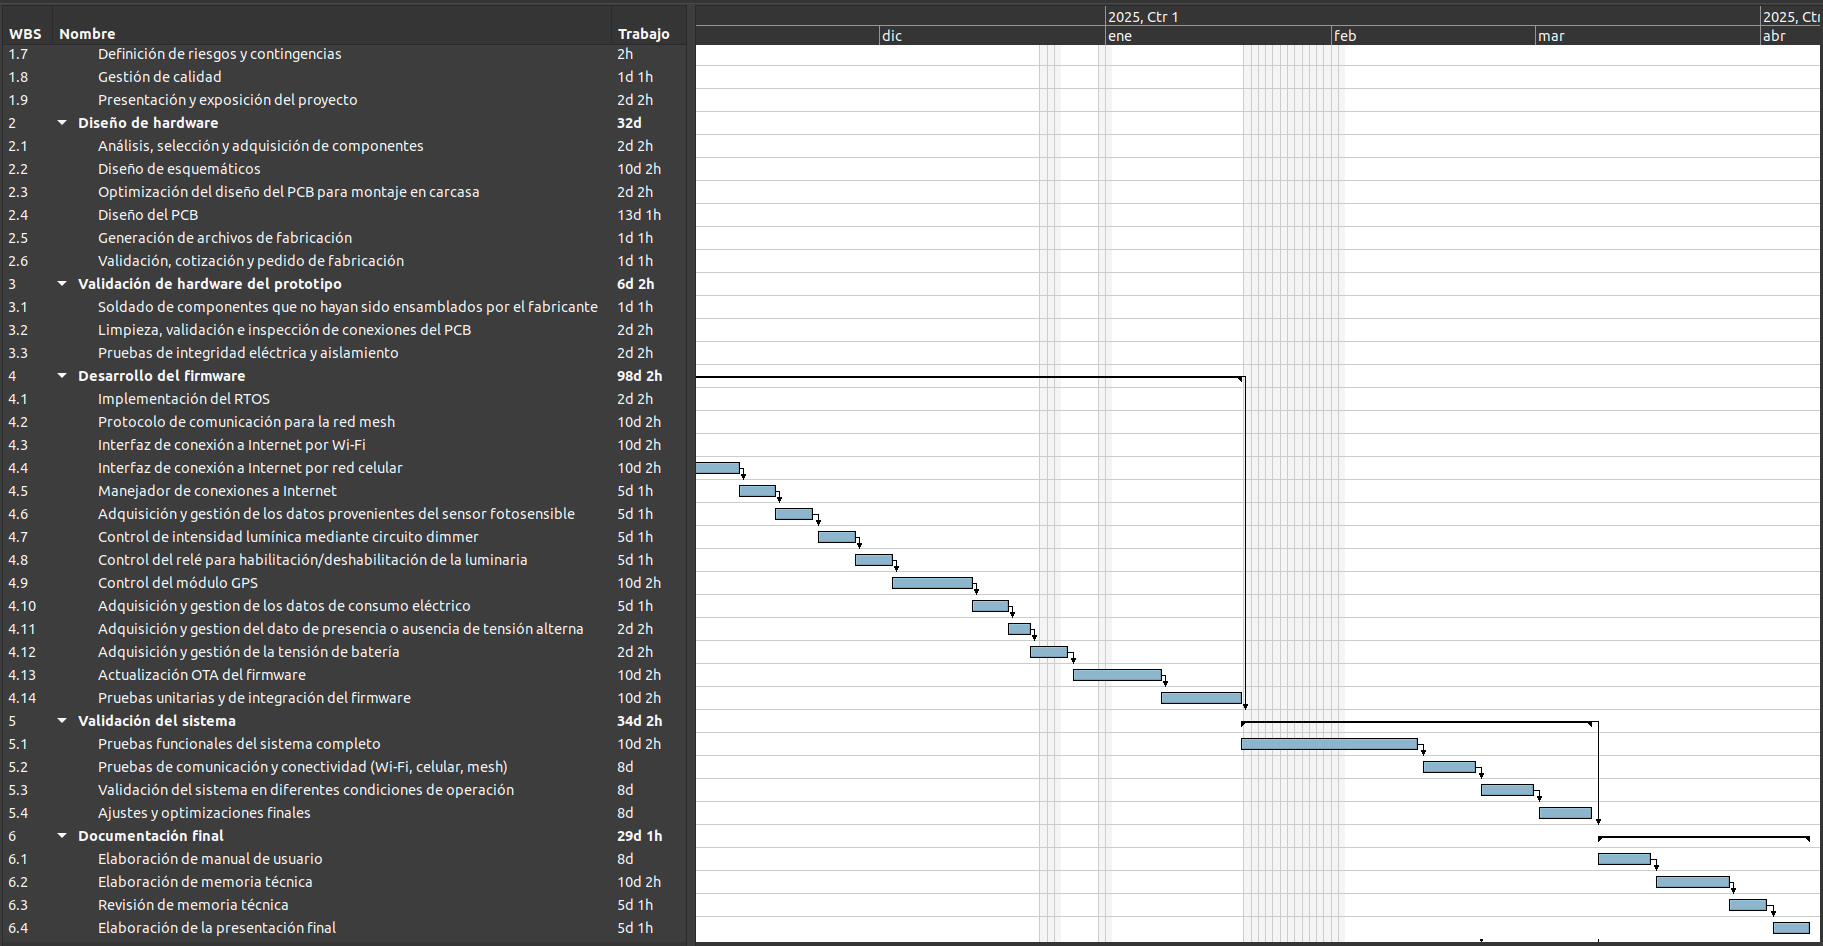
\includegraphics[height=.85\textheight]{./Figuras/Gantt-2.png}
\caption{Ejemplo de diagrama de Gantt (apaisado).} %Modificar este título acorde.
\label{fig:diagGantt}
\end{figure}

\end{landscape}

\end{consigna}


\section{12. Presupuesto detallado del proyecto}
\label{sec:presupuesto}

\begin{consigna}{red}
Si el proyecto es complejo entonces separarlo en partes:
\begin{itemize}
	\item Un total global, indicando el subtotal acumulado por cada una de las áreas.
	\item El desglose detallado del subtotal de cada una de las áreas.
\end{itemize}

IMPORTANTE: No olvidarse de considerar los COSTOS INDIRECTOS.

Incluir la aclaración de si se emplea como moneda el peso argentino (ARS) o si se usa moneda extranjera (USD, EUR, etc). Si es en moneda extranjera se debe indicar la tasa de conversión respecto a la moneda local en una fecha dada.

\end{consigna}

\begin{table}[htpb]
\centering
\begin{tabularx}{\linewidth}{@{}|X|c|r|r|@{}}
\hline
\rowcolor[HTML]{C0C0C0} 
\multicolumn{4}{|c|}{\cellcolor[HTML]{C0C0C0}COSTOS DIRECTOS} \\ \hline
\rowcolor[HTML]{C0C0C0} 
Descripción &
  \multicolumn{1}{c|}{\cellcolor[HTML]{C0C0C0}Cantidad} &
  \multicolumn{1}{c|}{\cellcolor[HTML]{C0C0C0}Valor unitario} &
  \multicolumn{1}{c|}{\cellcolor[HTML]{C0C0C0}Valor total} \\ \hline
 &
  \multicolumn{1}{c|}{} &
  \multicolumn{1}{c|}{} &
  \multicolumn{1}{c|}{} \\ \hline
 &
  \multicolumn{1}{c|}{} &
  \multicolumn{1}{c|}{} &
  \multicolumn{1}{c|}{} \\ \hline
\multicolumn{1}{|l|}{} &
   &
   &
   \\ \hline
\multicolumn{1}{|l|}{} &
   &
   &
   \\ \hline
\multicolumn{3}{|c|}{SUBTOTAL} &
  \multicolumn{1}{c|}{} \\ \hline
\rowcolor[HTML]{C0C0C0} 
\multicolumn{4}{|c|}{\cellcolor[HTML]{C0C0C0}COSTOS INDIRECTOS} \\ \hline
\rowcolor[HTML]{C0C0C0} 
Descripción &
  \multicolumn{1}{c|}{\cellcolor[HTML]{C0C0C0}Cantidad} &
  \multicolumn{1}{c|}{\cellcolor[HTML]{C0C0C0}Valor unitario} &
  \multicolumn{1}{c|}{\cellcolor[HTML]{C0C0C0}Valor total} \\ \hline
\multicolumn{1}{|l|}{} &
   &
   &
   \\ \hline
\multicolumn{1}{|l|}{} &
   &
   &
   \\ \hline
\multicolumn{1}{|l|}{} &
   &
   &
   \\ \hline
\multicolumn{3}{|c|}{SUBTOTAL} &
  \multicolumn{1}{c|}{} \\ \hline
\rowcolor[HTML]{C0C0C0}
\multicolumn{3}{|c|}{TOTAL} &
   \\ \hline
\end{tabularx}%
\end{table}


\section{13. Gestión de riesgos}
\label{sec:riesgos}

\begin{consigna}{red}
a) Identificación de los riesgos (al menos cinco) y estimación de sus consecuencias:
 
Riesgo 1: detallar el riesgo (riesgo es algo que si ocurre altera los planes previstos de forma negativa)
\begin{itemize}
	\item Severidad (S): mientras más severo, más alto es el número (usar números del 1 al 10).\\
	Justificar el motivo por el cual se asigna determinado número de severidad (S).
	\item Probabilidad de ocurrencia (O): mientras más probable, más alto es el número (usar del 1 al 10).\\
	Justificar el motivo por el cual se asigna determinado número de (O). 
\end{itemize}   

Riesgo 2:
\begin{itemize}
	\item Severidad (S): X.\\
	Justificación...
	\item Ocurrencia (O): Y.\\
	Justificación...
\end{itemize}

Riesgo 3:
\begin{itemize}
	\item Severidad (S):  X.\\
	Justificación...
	\item Ocurrencia (O): Y.\\
	Justificación...
\end{itemize}


b) Tabla de gestión de riesgos:      (El RPN se calcula como RPN=SxO)

\begin{table}[htpb]
\centering
\begin{tabularx}{\linewidth}{@{}|X|c|c|c|c|c|c|@{}}
\hline
\rowcolor[HTML]{C0C0C0} 
Riesgo & S & O & RPN & S* & O* & RPN* \\ \hline
       &   &   &     &    &    &      \\ \hline
       &   &   &     &    &    &      \\ \hline
       &   &   &     &    &    &      \\ \hline
       &   &   &     &    &    &      \\ \hline
       &   &   &     &    &    &      \\ \hline
\end{tabularx}%
\end{table}

Criterio adoptado: 

Se tomarán medidas de mitigación en los riesgos cuyos números de RPN sean mayores a...

Nota: los valores marcados con (*) en la tabla corresponden luego de haber aplicado la mitigación.

c) Plan de mitigación de los riesgos que originalmente excedían el RPN máximo establecido:
 
Riesgo 1: plan de mitigación (si por el RPN fuera necesario elaborar un plan de mitigación).
  Nueva asignación de S y O, con su respectiva justificación:
  \begin{itemize}
	\item Severidad (S*): mientras más severo, más alto es el número (usar números del 1 al 10).
          Justificar el motivo por el cual se asigna determinado número de severidad (S).
	\item Probabilidad de ocurrencia (O*): mientras más probable, más alto es el número (usar del 1 al 10).
          Justificar el motivo por el cual se asigna determinado número de (O).
	\end{itemize}

Riesgo 2: plan de mitigación (si por el RPN fuera necesario elaborar un plan de mitigación).
 
Riesgo 3: plan de mitigación (si por el RPN fuera necesario elaborar un plan de mitigación).

\end{consigna}


\section{14. Gestión de la calidad}
\label{sec:calidad}

\begin{consigna}{red}
Elija al menos diez requerimientos que a su criterio sean los más importantes/críticos/que aportan más valor y para cada uno de ellos indique las acciones de verificación y validación que permitan asegurar su cumplimiento.

\begin{itemize} 
\item Req \#1: copiar acá el requerimiento con su correspondiente número.

\begin{itemize}
	\item Verificación para confirmar si se cumplió con lo requerido antes de mostrar el sistema al cliente. Detallar.
	\item Validación con el cliente para confirmar que está de acuerdo en que se cumplió con lo requerido. Detallar. 
\end{itemize}

\end{itemize}

Tener en cuenta que en este contexto se pueden mencionar simulaciones, cálculos, revisión de hojas de datos, consulta con expertos, mediciones, etc.  

Las acciones de verificación suelen considerar al entregable como ``caja blanca'', es decir se conoce en profundidad su funcionamiento interno.  

En cambio, las acciones de validación suelen considerar al entregable como ``caja negra'', es decir, que no se conocen los detalles de su funcionamiento interno.

\end{consigna}

\section{15. Procesos de cierre}    
\label{sec:cierre}

\begin{consigna}{red}
Establecer las pautas de trabajo para realizar una reunión final de evaluación del proyecto, tal que contemple las siguientes actividades:

\begin{itemize}
	\item Pautas de trabajo que se seguirán para analizar si se respetó el Plan de Proyecto original:\\
	 - Indicar quién se ocupará de hacer esto y cuál será el procedimiento a aplicar. 
	\item Identificación de las técnicas y procedimientos útiles e inútiles que se emplearon, los problemas que surgieron y cómo se solucionaron:\\
	 - Indicar quién se ocupará de hacer esto y cuál será el procedimiento para dejar registro.
	\item Indicar quién organizará el acto de agradecimiento a todos los interesados, y en especial al equipo de trabajo y colaboradores:\\
	  - Indicar esto y quién financiará los gastos correspondientes.
\end{itemize}

\end{consigna}

\end{document}